\documentclass[tikz,border=12pt]{standalone}
% Estilo comum dos esquemas vetoriais das aulas da GA033.
\usepackage[T1]{fontenc}
\usepackage[utf8]{inputenc}
\usepackage{lmodern}
\usepackage{amsmath,amssymb}
\usetikzlibrary{arrows.meta,positioning,calc,fit,matrix,decorations.pathreplacing,backgrounds,shapes.geometric}
\definecolor{lnccblue}{HTML}{075AC0}
\definecolor{ink}{HTML}{242A31}
\definecolor{muted}{HTML}{647080}
\definecolor{lightblue}{HTML}{EFF5FC}
\definecolor{teal}{HTML}{197C83}
\definecolor{orange}{HTML}{BC6A16}
\tikzset{
  every node/.style={font=\sffamily\fontsize{15}{18}\selectfont,text=ink},
  box/.style={draw=lnccblue,line width=0.9pt,fill=lightblue,inner sep=9pt,align=center},
  flow/.style={-{Stealth[length=3mm,width=2mm]},draw=lnccblue,line width=1pt},
  point/.style={circle,draw=lnccblue,fill=white,line width=1.2pt,minimum size=3.2mm,inner sep=0pt},
  label/.style={font=\sffamily\fontsize{13}{16}\selectfont,text=muted},
  heading/.style={font=\sffamily\bfseries\fontsize{16}{19}\selectfont,text=lnccblue}
}
% Impede setas horizontais involuntariamente invertidas após editar os nós.
\newdimen\origemseta
\newdimen\destinoseta
\newcommand{\verificarsetadireita}[2]{%
  \pgfextractx{\origemseta}{\pgfpointanchor{#1}{east}}%
  \pgfextractx{\destinoseta}{\pgfpointanchor{#2}{west}}%
  \advance\origemseta by 4mm%
  \ifdim\destinoseta>\origemseta\else
    \PackageError{diagramas}{Conector sem espaco entre #1 e #2}{Afaste os nos antes de compilar.}%
  \fi
}

\begin{document}
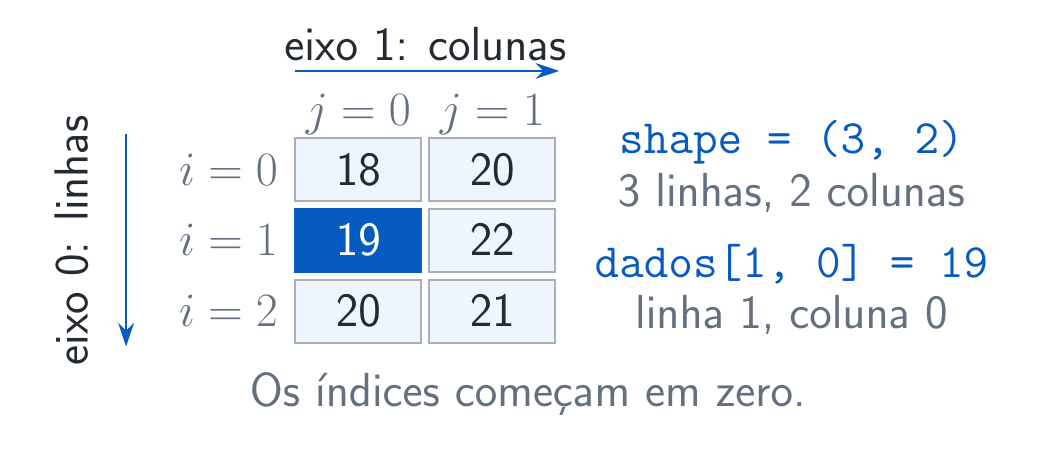
\begin{tikzpicture}[x=1cm,y=1cm,
  every node/.append style={font=\sffamily\fontsize{16}{19}\selectfont},
  cell/.style={draw=muted!55,line width=.7pt,minimum width=1.6cm,minimum height=.8cm,inner sep=0pt}]
  \path[use as bounding box] (0,0) rectangle (12.5,5.0);
  \draw[flow] (3.4,4.45) -- (6.75,4.45);
  \node at (5.05,4.8) {eixo 1: colunas};
  \draw[flow] (1.25,3.65) -- (1.25,.95);
  \node[rotate=90] at (.55,2.3) {eixo 0: linhas};
  \node[text=muted] at (4.2,3.9) {$j=0$};
  \node[text=muted] at (5.9,3.9) {$j=1$};
  \node[text=muted] at (2.55,3.2) {$i=0$};
  \node[text=muted] at (2.55,2.3) {$i=1$};
  \node[text=muted] at (2.55,1.4) {$i=2$};
  \node[cell,fill=lightblue] at (4.2,3.2) {18};
  \node[cell,fill=lightblue] at (5.9,3.2) {20};
  \node[cell,draw=lnccblue,fill=lnccblue,text=white] at (4.2,2.3) {19};
  \node[cell,fill=lightblue] at (5.9,2.3) {22};
  \node[cell,fill=lightblue] at (4.2,1.4) {20};
  \node[cell,fill=lightblue] at (5.9,1.4) {21};
  \node[heading] at (9.7,3.55) {\texttt{shape = (3, 2)}};
  \node[text=muted] at (9.7,2.9) {3 linhas, 2 colunas};
  \node[text=lnccblue] at (9.7,2.0) {\texttt{dados[1, 0] = 19}};
  \node[text=muted] at (9.7,1.35) {linha 1, coluna 0};
  \node[text=muted] at (6.35,.35) {Os índices começam em zero.};
\end{tikzpicture}
\end{document}
